\documentclass[conference]{IEEEtran}

\usepackage[T1]{fontenc}
\usepackage{amsmath,amssymb}
\usepackage{graphicx}
\usepackage{booktabs}
\usepackage{array}
\usepackage{cite}
\usepackage{url}

\makeatletter
\newcommand{\setR}[2]{\expandafter\def\csname R@#1\endcsname{#2}}
\newcommand{\R}[1]{\ifcsname R@#1\endcsname\csname R@#1\endcsname\else\textit{(pending)}\fi}
\makeatother
\InputIfFileExists{../report/generated/numbers.tex}{}{}

\newcommand{\drtc}{DRTC}
\newcommand{\smolvla}{SmolVLA}
\newcommand{\groot}{GR00T~N1.5}
\newcommand{\pizerofive}{$\pi_{0.5}$}
\newcommand{\pending}{\textit{(pending)}}
\newcommand{\jerkunit}{$10^3\,^\circ/\mathrm{s}^3$}

\begin{document}

\title{Evaluating Distributed Real-Time Chunking and Motion Smoothing for Remote Robot Policy Inference}

\author{\IEEEauthorblockN{Author names to be added}}

\maketitle

\begin{abstract}
Large vision-language-action and action-chunking policies often require GPU servers, forcing low-cost robots such as the SO-101 arm to rely on remote inference over wireless links. When network replies are delayed or lost, the client shipped with LeRobot~0.7 ends runs after one second of queue starvation and replaces a lost request only once its queue has run dry. We port Distributed Real-Time Chunking (\drtc{}) into LeRobot~0.7 with four fixes discovered under slow links and short chunks, implement six smoothing methods and seven injectable network faults, and build a replay bench to evaluate seven policies across two manipulation tasks. In a first robot study on sorting (\R{main/n} trials), faults reduced shipped-client success to \R{main/smolvla/faults/M1} and \R{main/groot/faults/M1}, whereas \drtc{} achieved \R{main/smolvla/drtc/M1} (\smolvla{}) and \R{main/groot/drtc/M1} (\groot{}). Against a patient baseline on the bench (\R{v2/sort_one/e1/n} sorting runs in E1--E2), \drtc's cooldown re-request drives recovery from drops and outages, though it stalls more under rising latency, and smoothing cuts jerk 3--20$\times$.
\end{abstract}

\begin{IEEEkeywords}
remote inference, action chunking, network faults, real-time chunking, motion smoothing, SO-101.
\end{IEEEkeywords}

\section{Introduction}

Imitation learning policies can now acquire tabletop manipulation skills from a few dozen demonstrations~\cite{zhao2023act,chi2023diffusion}. Recent vision-language-action (VLA) models, including \smolvla~\cite{shukor2025smolvla}, the GR00T family~\cite{nvidia2025gr00t}, \pizerofive~\cite{pi2025pi05}, and MolmoAct~2~\cite{molmoact2}, extend this paradigm with pretrained vision-language backbones ranging from roughly half a billion to several billion parameters. Because low-cost arms such as the SO-101~\cite{so101} are driven by laptops or single-board computers, these policies typically run via \emph{remote inference}: the robot sends camera images and joint states over the network to a GPU server and receives a chunk of future actions executed at 30~Hz.

Sending multi-step chunks allows execution and inference to overlap~\cite{shukor2025smolvla}, but it leaves every run dependent on an unreliable wireless link. WiFi links exhibit latency spikes, packet drops, and brief disconnects. When a reply arrives late or is lost, the client's action queue empties and the arm stalls. In LeRobot~0.7~\cite{lerobot}, the shipped remote-inference client terminates a run after 1~s without actions and never re-requests a lost reply, causing even transient faults to abort tasks.

Distributed Real-Time Chunking (\drtc)~\cite{vial2026drtc} addresses this fragility by triggering chunk requests early, estimating round-trip time via a TCP-style estimator, and re-requesting with a fresh observation when an overdue reply exceeds a cooldown. However, \drtc{} had not been independently evaluated against LeRobot's client on task success under controlled faults, ablated to isolate which mechanisms matter, or paired with systematic motion smoothing across policies with differing chunk lengths.

This paper condenses our implementation and empirical evaluation on an SO-101 arm and a seven-policy replay bench. Our contributions are:
\begin{enumerate}
  \item \textbf{\drtc{} on LeRobot~0.7 with four fixes:} an integration inside LeRobot's shipped runtime with four repairs for failures exposed by slow links and short action chunks.
  \item \textbf{Fault injection and replay bench:} seven deterministic, trial-shifted network fault profiles and a hardware-in-the-loop replay plugin simulating measured WiFi latency across held-out episodes.
  \item \textbf{Robot and seven-policy bench evaluation:} physical robot trials on sorting and \R{v2/sort_one/e1/n} sorting bench runs across seven policies comparing \drtc{} against shipped and patient baselines, plus component ablations.
  \item \textbf{Pre-registered smoothing study:} six smoothing methods tested individually and combined via a pre-registered selection rule guarding against plan lag, revealing when guided real-time chunking hurts on network-bound links.
\end{enumerate}

\section{Background and Related Work}

\subsection{Action Chunking and Policies}

Predicting single actions makes visuomotor policies vulnerable to compounding errors and inference jitter. Action chunking instead predicts $H$ future actions $A_t = (a_t,\dots,a_{t+H-1})$ per observation~\cite{zhao2023act}. Targets may be absolute joint angles or relative to the current state; relative actions generalize across poses but bind a chunk to its originating state.

Published SO-101 benchmarks report wide performance gaps across policy families~\cite{armnetbench,so101failure,valloss2026} and show that trimming idle episode starts removes most ``never started'' failures~\cite{valloss2026}. Following this evidence, we train seven policies spanning small models and large VLAs: ACT ($H=100$, absolute)~\cite{zhao2023act}, Diffusion Policy ($H=48$, 24 executed, absolute)~\cite{chi2023diffusion}, \smolvla{} ($\approx$0.45B, $H=50$, absolute)~\cite{shukor2025smolvla}, \groot{} (3B, $H=16$, absolute)~\cite{nvidia2025gr00t}, GR00T~N1.7 (3B, $H=16$, relative arm)~\cite{nvidia2025gr00t}, \pizerofive{} ($\approx$3.4B, $H=50$, relative)~\cite{pi2025pi05}, and MolmoAct~2 ($H=30$, absolute)~\cite{molmoact2}. For remote inference, chunk length $H$ is critical: a 16-action chunk lasts only 0.53~s at 30~Hz, leaving almost no buffer over a WiFi round trip.

\subsection{Remote Inference, RTC, and DRTC}

Asynchronous client-server inference overlaps action execution with server computation~\cite{shukor2025smolvla}, implemented in LeRobot~0.7 over Zenoh. Because consecutive chunks are predicted from different observations, chunk boundaries can disagree and cause sudden jumps. Real-Time Chunking (RTC)~\cite{black2025rtc} mitigates boundary seams by treating flow-matching generation as in-painting, fixing the prefix of actions still executing from the current chunk while computing the new one.

\drtc{}~\cite{vial2026drtc} couples asynchronous execution with fault resilience through four mechanisms: (i) an early request trigger when queued steps drop to $H - s_{\min}$; (ii) Jacobson--Karels round-trip estimation~\cite{jacobson1988congestion,rfc6298}; (iii) a cooldown timeout that abandons overdue requests and sends a fresh observation; and (iv) last-write-wins register semantics from conflict-free replicated data types (CRDTs)~\cite{shapiro2011crdt} to discard stale or reordered replies.

\subsection{Command Smoothing}

Abrupt action transitions excite arm mechanics. Causal low-pass filters such as Butterworth filters~\cite{butterworth1930} attenuate high-frequency jitter at the cost of phase lag, whereas forward-backward zero-phase filtering~\cite{gustafsson1996} avoids delay when future samples are known in the queue. Chunk-specific techniques include temporal ensembling across overlapping chunks~\cite{zhao2023act}, adaptive playback speed during queue depletion, and minimum-jerk blending~\cite{flash1985} when restarting after a stall.

\section{System}

\subsection{Platform, Hardware, and Control Loop}

Our software layer sits cleanly on top of unmodified LeRobot~0.7~\cite{lerobot}, covered by \R{software/tests} automated tests, and adds two plugins: a \groot{} policy plugin with guided RTC (removed upstream after LeRobot~0.5.1) and a replay-robot driver. An experiment registry pins hardware rigs, Hugging Face Hub dataset revisions, training recipes, model commits, and study plans.

The physical rig uses a 6-DOF SO-101 follower arm~\cite{so101} (Feetech servos in degrees) and an identical leader arm for teleoperation. Two $800\times 600$ cameras---a wrist camera on the gripper and a fixed scene camera---capture at 30~fps. The robot computer (a Linux laptop with an RTX~4060 GPU; or a Raspberry~Pi~5 in an edge test) runs the 30~Hz control loop ($\Delta = 1/30$~s) and connects over WiFi and an SSH tunnel to shared NVIDIA A100 (80~GB) and H200 (141~GB) servers. Every observation transmits both uncompressed images ($\approx$2.9~MB) plus six joint positions.

When a scheduler requests a chunk, the server returns $H$ actions into the client's queue; at each tick, one action passes through smoothing to the arm. If the queue empties before a reply arrives, the arm holds its last commanded pose (a \emph{stall}). In an uncounted edge feasibility test on a Raspberry~Pi~5 over the laptop's hotspot, the control loop held \R{edge/hz} with no dropped frames, though round-trip times roughly doubled (\R{edge/smolvla/rtt} for \smolvla{}, \R{edge/groot/rtt} for \groot{}), causing \groot's 0.53~s queue to empty even without faults.

\subsection{Upstream Baseline vs.\ DRTC}

LeRobot~0.7's shipped client (\emph{upstream}) keeps at most one request in flight and triggers when queued playback time $q_t\,\Delta$ satisfies
\begin{equation}
  q_t\,\Delta \;\le\; \max\!\left(T_{\mathrm{refill}},\; \hat{L} + \Delta\right),
\end{equation}
where $T_{\mathrm{refill}}=0.5$~s and $\hat{L}$ is the maximum of the last 100 measured turnarounds. It enforces a 1~s \emph{starvation grace} (ending the run after 1~s with an empty queue and discarding the in-flight request once the queue empties) and a 5~s \emph{request deadline}, never re-requesting a lost reply. In addition to \emph{as shipped}, we define a \emph{patient} upstream baseline with both limits raised to the full trial duration so it never self-terminates.

We implemented \drtc{} inside LeRobot's runtime, preserving all upstream safety checks and using the same whole-trial limits as patient upstream:
\begin{itemize}
  \item \textbf{Trigger:} Request when $q_t \le H - s_{\min}$, with $s_{\min}=20$ steps for 50-action policies (\smolvla{} triggers with 30 actions / 1~s remaining vs.\ 0.5~s upstream) and $s_{\min}=8$ for 16- and 24-action policies.
  \item \textbf{Latency estimator:} For each measured turnaround $R$, update mean $\bar{R}$ and mean deviation $D$ via Jacobson--Karels~\cite{rfc6298}:
  \begin{equation}
    D \leftarrow (1-\beta)D + \beta|R-\bar{R}|,\quad
    \bar{R} \leftarrow (1-\alpha)\bar{R} + \alpha R,\quad
    \hat{L} = \bar{R} + kD,
  \end{equation}
  with $\alpha=1/8$, $\beta=1/4$, and $k=1.5$.
  \item \textbf{Cooldown re-request:} Abandon an unanswered request after cooldown $c$ and send a fresh observation (last-write-wins discards stale replies):
  \begin{equation}
    c = \max\!\left(2,\; \left\lceil \tilde{L}/\Delta \right\rceil + \varepsilon\right)\Delta,\quad
    \tilde{L} = \max\!\left(\hat{L},\; \max_{i\in \text{last }10} R_i\right),
  \end{equation}
  with $\varepsilon=1$, and initial pre-reply timeout $\max((s_{\min}+\varepsilon)\Delta, T_{\mathrm{start}})$ where $T_{\mathrm{start}}=10$~s.
\end{itemize}

\subsection{Four Fixes Found on the Real Setup}

Running \drtc{} on the physical rig and replay bench revealed four failure modes, summarized in Table~\ref{tab:fixes}. Removing the $H/2$ cooldown cap was essential for short-chunk models whose round trip exceeded half a chunk, while tracking the slowest of the last 10 replies prevented re-request storms from overloading the server.

\begin{table}[t]
  \centering
  \caption{DRTC failure modes observed on the real setup and our fixes.}
  \label{tab:fixes}
  \footnotesize
  \begin{tabular}{@{}p{0.26\columnwidth}p{0.34\columnwidth}p{0.31\columnwidth}@{}}
    \toprule
    Failure & Cause & Fix \\
    \midrule
    \groot{} received no chunks & $H/2$ cooldown cap (8 steps / 0.27~s) $<$ 0.4--0.7~s RTT & Remove $H/2$ cap (kept as ablation A4) \\
    Re-request storm & Near-estimate replies timed out; server stayed busy & Floor $\tilde{L}$ by max of last 10 replies \\
    No start on slow link & Pre-reply cooldown only $s_{\min}+\varepsilon$ steps & Wait up to $T_{\mathrm{start}}=10$~s before first reply \\
    ``Invalid RTC delay'' & Requested delay exceeded server chunk length & Cap delay at server prediction steps \\
    \bottomrule
  \end{tabular}
\end{table}

\subsection{Motion Smoothing}

We identify four sources of jerky motion: chunk \emph{seams}, queue \emph{stalls}, intra-chunk \emph{jitter}, and \emph{fault restarts}. We implemented six methods:
\begin{itemize}
  \item \textbf{Butterworth filter} (jitter, seams; all policies): causal 2nd-order low-pass per joint (3~Hz cutoff at 30~Hz) with amplitude gain $g=1.4$: $u_t = u_{t-1} + g(y_t - u_{t-1})$, reset on invalidation.
  \item \textbf{Zero-lag queue smoothing} (jitter; all policies): forward-backward Butterworth filtering~\cite{gustafsson1996} over the last $h=15$ executed steps and the accepted queue.
  \item \textbf{RTC} (seams; flow-matching absolute policies: \smolvla{}, \groot{}): guided denoising conditioned on queued prefix actions~\cite{black2025rtc}, after one uncounted warm-up round to compile the guided path.
  \item \textbf{Temporal ensembling} (seams; all policies): exponential weighting $w_i = e^{-0.01\,i}$ over overlapping chunk predictions at the queue cursor~\cite{zhao2023act}.
  \item \textbf{Adaptive playback} (stalls; all policies): scales phase increment $r_t \in [0.5,1.0]$ toward $q_t/(n_t+4)$ (slew limit $\sigma=0.05$/tick) with linear interpolation when $n_t$ expected ticks remain until arrival.
  \item \textbf{Resume ramp} (restarts; all policies): after a stall $\ge 0.1$~s, blends $N=10$ commands from held pose $p_0$ using a minimum-jerk profile $w(\tau)=10\tau^3-15\tau^4+6\tau^5$~\cite{flash1985}.
\end{itemize}
An early \emph{soft stop} decelerated before queue exhaustion, but kept the queue alive long enough to accept a 1.3~s stale observation on \smolvla{}, spiking the next step to 38--42$^\circ$ (vs.\ 18$^\circ$ for \drtc{} alone); it was dropped.

\subsection{Fault Injection and Replay Bench}

Faults are injected directly in the client transport so all deadlines and recovery logic respond naturally: \emph{none} (fault-free); \emph{spike} (one reply delayed 1~s at $t=2$~s); \emph{drops} (all replies lost over 4--5~s); \emph{outage} (both directions lost over 6--7.5~s); \emph{mix} (spike, drops, and outage); \emph{rise} (+400~ms latency from 2 to 7~s); and \emph{loss} (10\% independent reply loss). In setup~v2, timed faults are shifted per trial by a deterministic offset drawn uniformly from 0--4~s (seeded by trial index) so faults hit reach, grasp, and place phases uniformly across conditions.

The \emph{replay bench} replaces the physical arm with our replay-robot plugin streaming held-out recorded episodes to a policy server on the same GPU machine, while injecting 250~ms ($\pm$20~ms jitter) baseline network latency matching robot measurements. Runs dropping below 27~Hz are excluded. While the bench cannot measure task success (images do not react to actions), it isolates timing, stalls, recovery, and motion across all policies and faults without operator bottleneck.

\section{Evaluation Design}

\subsection{Datasets and Trained Policies}

We recorded two tasks at 30~fps on the SO-101 arm, planning held-out splits upfront and automatically trimming idle start/end frames~\cite{valloss2026}: \emph{cube in box v1} (100 train + 10 held-out episodes; 25{,}067 frames; normalized units $-100$..$100$, following an initial 50-episode v0 set) and \emph{sorting} (80 train + 8 held-out episodes; 20{,}935 frames; degrees), where a red or blue cube is placed into a matching square whose side alternates across four balanced layouts. All seven policies were trained on both datasets using authors' unmodified recipes (stopping \pizerofive{} at 15k/20k and MolmoAct~2 at 30k/50k steps for time).

\subsection{First Robot Run and Redesign to Setup v2}

A first robot study on sorting (10 trials/cell, unshifted faults) tested \smolvla{} and \groot{} under four conditions: (1) shipped baseline (normal network), (2) shipped baseline + fault mix, (3) \drtc{} + mix, and (4) \drtc{} + smoothing (Butterworth + adaptive playback) + mix. Because condition~2 terminated every trial at the first fault via its 1~s starvation grace, it confounded scheduling with patience and coupled two smoothing methods at once.

We therefore designed \emph{setup~v2}, pairing \drtc{} against the \emph{patient} upstream baseline with identical whole-trial limits across four bench studies (8 runs/cell, 14~s each, 52 shared conditions per task in E1--E2) and one robot study:
\begin{itemize}
  \item \textbf{E1 (Bench, 7 policies $\times$ 2 tasks):} patient upstream, shipped upstream, and \drtc{} across all seven fault types.
  \item \textbf{E2 (Bench ablations):} \drtc{} without cooldown (A1), with upstream's latency estimator (A2), with upstream's trigger (A3), and with the original $H/2$ cap (A4); runs with $0.5\times$ and $1.5\times$ $s_{\min}$ (A5) are not yet analysed.
  \item \textbf{E3a/E3b (Bench smoothing):} each smoothing method alone under the mix (E3a), followed by the pre-registered stack and leave-one-out ablations (E3b).
  \item \textbf{E4 (Robot, pending):} 10 sorting trials/cell for \smolvla{} and \groot{} comparing fault-free patient upstream against patient, \drtc{}, and \drtc{}+stack under the mix.
\end{itemize}

\subsection{Metrics, Pre-Registration, and Stack Selection}

Every study freezes model Hub commits and analysis plans before trial~1, executes in seeded randomized rounds per layout, logs raw per-tick and per-chunk records, and reads fault termination labels from system logs rather than operator keys. Primary metrics (version~3) are: success rate \textbf{M1} (with Wilson 95\% intervals~\cite{wilson1927}), fault-ended trials \textbf{M1f}, time to success \textbf{M1t}, stall fraction \textbf{M2} (ticks without a new action after first movement), turnaround/inference/estimate error \textbf{M4--M6}, RMS moving-only joint jerk \textbf{M7} (\jerkunit{}, excluding stationary ticks so stalling does not appear smooth), largest step \textbf{M8}, offline held-out MAE and inference cost \textbf{M9--M10}, per-fault recovery time \textbf{M11} (fault end until arm moves, or unrecovered), and deviation from the policy's raw plan \textbf{M12}.

Primary comparisons are tested via Fisher's exact test~\cite{fisher1935} (M1) and two-sided Mann--Whitney $U$ tests~\cite{mann1947} with Holm correction~\cite{holm1979}. For E3a, a pre-registered script selects the stack from adaptive playback, resume ramp, one seam method (RTC vs.\ ensembling), and one jitter method (Butterworth vs.\ zero-lag): candidates exceeding 1$^\circ$ median M12 deviation, raising median M2 or M11 by $>10\%$ (minimum 0.5~pp / 0.05~s), or reducing recovered runs are disqualified; remaining candidates win by lower M7 jerk, and the method winning more policy-task pairs is chosen.

\section{Results}

The first robot run, its single-fault benches, offline evaluations (four policies), and setup~v2 bench studies E1 and E2 on sorting and E3a--E3b on both tasks are complete; E1 and E2 on cube in box, E4 and the seven-policy robot baselines remain \pending.

\subsection{First Robot Run, Single-Fault Benches, and Offline Cost}

On the physical sorting task (\R{main/n} valid trials across \R{main/sessions} sessions; \R{main/notcounted} trial excluded before first action due to a motor-bus fault), faults destroyed the shipped client (Fig.~\ref{fig:main_success}, Table~\ref{tab:main_summary}). Success dropped from \R{main/smolvla/baseline/M1} to \R{main/smolvla/faults/M1} on \smolvla{} (\R{main/smolvla/p/baseline-faults/M1}) and from \R{main/groot/baseline/M1} to \R{main/groot/faults/M1} on \groot{} (\R{main/groot/p/baseline-faults/M1}), with \R{main/smolvla/faults/M1f} and \R{main/groot/faults/M1f} ended at the initial latency spike. \drtc{} eliminated fault terminations (\R{main/smolvla/drtc/M1f}, \R{main/groot/drtc/M1f}) and restored success to \R{main/smolvla/drtc/M1} (\R{main/smolvla/p/faults-drtc/M1}) and \R{main/groot/drtc/M1} (\R{main/groot/p/faults-drtc/M1}), recovering motion after every fault, at most 1.45~s (median) after its end (\groot{} outage: \R{main/groot/drtc/M11/outage}). Single-fault bench runs replicated this pattern: each fault alone caused \R{bench/spike/smolvla/faults/M1f} (spike), \R{bench/drops/smolvla/faults/M1f} (drops), and \R{bench/outage/smolvla/faults/M1f} (outage) terminations on \smolvla{} for the shipped client, versus \R{bench/mix/smolvla/drtc/M1f} and \R{bench/mix/groot/drtc/M1f} under the mix with \drtc{}.

\begin{figure}[t]
  \centering
  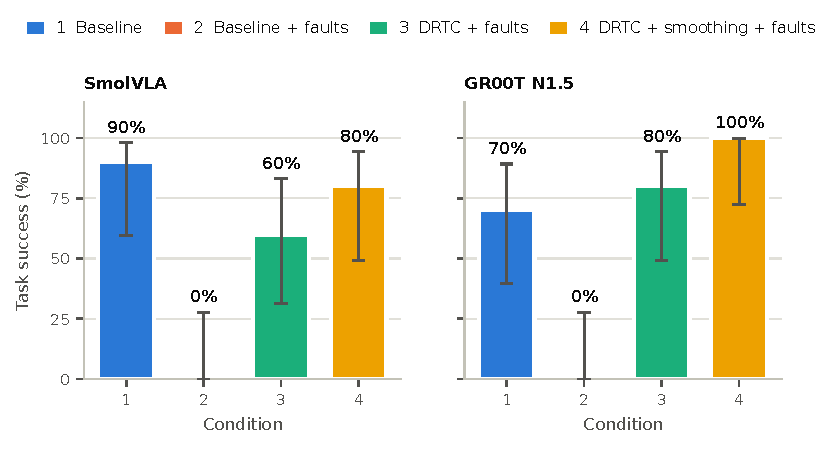
\includegraphics[width=\columnwidth]{../report/generated/fig_main_success.pdf}
  \caption{First robot run on sorting: task success with Wilson 95\% intervals ($n=10$ trials per bar). Condition~2 failed every trial at the first fault.}
  \label{fig:main_success}
\end{figure}

\begin{table}[t]
  \centering
  \caption{First robot run on sorting ($n=10$ per condition; medians for M2, M7, M8).}
  \label{tab:main_summary}
  \footnotesize
  \begin{tabular}{@{}llccccc@{}}
    \toprule
    Policy & Condition & M1 (95\% CI) & M1f & M2 & M7 & M8 \\
    \midrule
    \smolvla & 1 Baseline & \R{main/smolvla/baseline/M1} (\R{main/smolvla/baseline/M1ci}) & \R{main/smolvla/baseline/M1f} & \R{main/smolvla/baseline/M2} & \R{main/smolvla/baseline/M7} & \R{main/smolvla/baseline/M8b} \\
             & 2 + faults & \R{main/smolvla/faults/M1} (\R{main/smolvla/faults/M1ci}) & \R{main/smolvla/faults/M1f} & \R{main/smolvla/faults/M2} & \R{main/smolvla/faults/M7} & \R{main/smolvla/faults/M8b} \\
             & 3 \drtc{} + faults & \R{main/smolvla/drtc/M1} (\R{main/smolvla/drtc/M1ci}) & \R{main/smolvla/drtc/M1f} & \R{main/smolvla/drtc/M2} & \R{main/smolvla/drtc/M7} & \R{main/smolvla/drtc/M8b} \\
             & 4 + smooth & \R{main/smolvla/smooth/M1} (\R{main/smolvla/smooth/M1ci}) & \R{main/smolvla/smooth/M1f} & \R{main/smolvla/smooth/M2} & \R{main/smolvla/smooth/M7} & \R{main/smolvla/smooth/M8b} \\
    \addlinespace
    \groot   & 1 Baseline & \R{main/groot/baseline/M1} (\R{main/groot/baseline/M1ci}) & \R{main/groot/baseline/M1f} & \R{main/groot/baseline/M2} & \R{main/groot/baseline/M7} & \R{main/groot/baseline/M8b} \\
             & 2 + faults & \R{main/groot/faults/M1} (\R{main/groot/faults/M1ci}) & \R{main/groot/faults/M1f} & \R{main/groot/faults/M2} & \R{main/groot/faults/M7} & \R{main/groot/faults/M8b} \\
             & 3 \drtc{} + faults & \R{main/groot/drtc/M1} (\R{main/groot/drtc/M1ci}) & \R{main/groot/drtc/M1f} & \R{main/groot/drtc/M2} & \R{main/groot/drtc/M7} & \R{main/groot/drtc/M8b} \\
             & 4 + smooth & \R{main/groot/smooth/M1} (\R{main/groot/smooth/M1ci}) & \R{main/groot/smooth/M1f} & \R{main/groot/smooth/M2} & \R{main/groot/smooth/M7} & \R{main/groot/smooth/M8b} \\
    \bottomrule
  \end{tabular}
\end{table}

Adding Butterworth + adaptive playback in condition~4 cut jerk from \R{main/smolvla/drtc/M7} to \R{main/smolvla/smooth/M7}~\jerkunit{} (\R{main/smolvla/jerkratio}$\times$, \R{main/smolvla/p/drtc-smooth/M7}) on \smolvla{} and from \R{main/groot/drtc/M7} to \R{main/groot/smooth/M7} (\R{main/groot/jerkratio}$\times$, \R{main/groot/p/drtc-smooth/M7}) on \groot{}, while reducing largest steps (\R{main/smolvla/drtc/M8b} to \R{main/smolvla/smooth/M8b}; \R{main/groot/drtc/M8b} to \R{main/groot/smooth/M8b}) and cutting \groot{} stalls from \R{main/groot/drtc/M2} to \R{main/groot/smooth/M2} (\R{main/groot/p/drtc-smooth/M2}) without lowering success (\R{main/smolvla/smooth/M1}, \R{main/groot/smooth/M1}). Normal-network median turnaround was \R{main/smolvla/baseline/M4med} (\R{main/smolvla/baseline/M6} server, \R{main/smolvla/baseline/net} network) for \smolvla{} and \R{main/groot/baseline/M4med} (\R{main/groot/baseline/M6} server, \R{main/groot/baseline/net} network) for \groot{}. On a shared \R{offline/gpu}, offline sorting arm-joint MAE was lowest for \smolvla{} (\R{offline/sortone/smolvla/M9arm}$^\circ$), followed by Diffusion Policy (\R{offline/sortone/diffusion/M9arm}$^\circ$), \groot{} (\R{offline/sortone/groot/M9arm}$^\circ$), and ACT (\R{offline/sortone/act/M9arm}$^\circ$; fastest at \R{offline/sortone/act/M10}, \R{offline/sortone/act/M10gb}, vs.\ \R{offline/sortone/groot/M10gb} for \groot{}).

\subsection{Setup v2: DRTC vs.\ Patient Upstream and Ablations (E1, E2)}

Across \R{v2/sort_one/e1/n} sorting bench runs of the E1--E2 plan (Fig.~\ref{fig:v2_e1}), fault-free stalls were similar between \drtc{} and patient upstream, except MolmoAct~2 (\R{v2/sort_one/e1/none/molmoact2/drtc}\,\% vs.\ \R{v2/sort_one/e1/none/molmoact2/patient}\,\%). Under faults with lost replies, \drtc{} sharply outperformed waiting: under the mix, stalls fell from \R{v2/sort_one/e1/mix/act/patient}\,\% to \R{v2/sort_one/e1/mix/act/drtc}\,\% (ACT), \R{v2/sort_one/e1/mix/smolvla/patient}\,\% to \R{v2/sort_one/e1/mix/smolvla/drtc}\,\% (\smolvla{}), and \R{v2/sort_one/e1/mix/pi05/patient}\,\% to \R{v2/sort_one/e1/mix/pi05/drtc}\,\% (\pizerofive{}). \drtc{} recovered all 24 fault events in six of seven policies (GR00T~N1.7: \R{v2/sort_one/e1/mix/grootn17/drtcrec}), versus \R{v2/sort_one/e1/mix/smolvla/patientrec} (\smolvla{}) and \R{v2/sort_one/e1/mix/groot/patientrec} (\groot{}) for patient upstream. After an outage, patient upstream recovered in \R{v2/sort_one/e1/outage/smolvla/patientrec} \smolvla{} and \R{v2/sort_one/e1/outage/groot/patientrec} \groot{} runs---because it re-requests only once when its queue empties and stalls until the 10~s deadline if that request drops---whereas \drtc{} recovered 8/8 runs in \R{v2/sort_one/e1/outage/smolvla/drtcrectime}\,s and \R{v2/sort_one/e1/outage/groot/drtcrectime}\,s. Both clients absorbed single spikes.

\begin{figure*}[t]
  \centering
  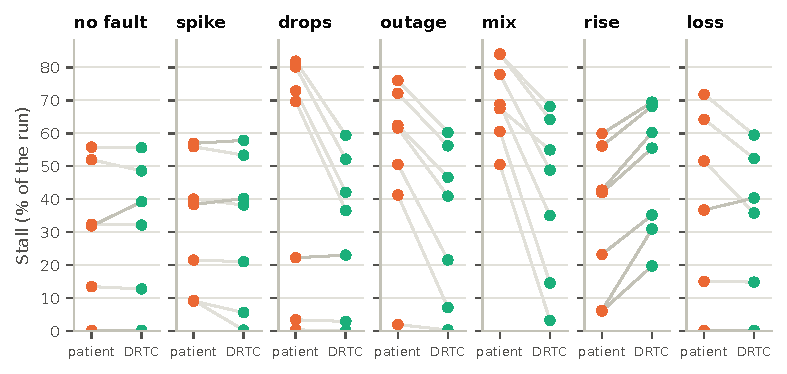
\includegraphics[width=0.92\textwidth]{../report/generated/fig_v2_e1_sort_one.pdf}
  \caption{Setup v2 E1 on sorting: median stall fraction across all seven policies under patient upstream (orange) and \drtc{} (green) per fault type. \drtc{} cuts stalls under drops, outages, and the mix, but stalls more than patient upstream for every policy under rising latency (\emph{rise}).}
  \label{fig:v2_e1}
\end{figure*}

Crucially, \drtc{} was consistently \emph{worse} than patient upstream under \emph{rise} (+400~ms for 5~s) across all seven policies---for example \R{v2/sort_one/e1/rise/smolvla/drtc}\,\% vs.\ \R{v2/sort_one/e1/rise/smolvla/patient}\,\% on \smolvla{} and \R{v2/sort_one/e1/rise/act/drtc}\,\% vs.\ \R{v2/sort_one/e1/rise/act/patient}\,\% on ACT. Because the cooldown tracks recent faster replies, it aborts responses that are merely slower than before; the server, still computing the abandoned request, returns BUSY and delays the replacement.

\begin{table}[t]
  \centering
  \caption{E2 ablations on sorting against \drtc{} (policies with higher stalls and median $\Delta$ in percentage points).}
  \label{tab:e2}
  \footnotesize
  \begin{tabular}{@{}llcc@{}}
    \toprule
    Ablation & Fault & Worse policies & Median $\Delta$ (pp) \\
    \midrule
    A1 no cooldown          & mix    & \R{v2/sort_one/e2/a1_no_cooldown/mix/worse} & \R{v2/sort_one/e2/a1_no_cooldown/mix/delta} \\
                            & outage & \R{v2/sort_one/e2/a1_no_cooldown/outage/worse} & \R{v2/sort_one/e2/a1_no_cooldown/outage/delta} \\
                            & drops  & \R{v2/sort_one/e2/a1_no_cooldown/drops/worse} & \R{v2/sort_one/e2/a1_no_cooldown/drops/delta} \\
                            & rise   & \R{v2/sort_one/e2/a1_no_cooldown/rise/worse} & \R{v2/sort_one/e2/a1_no_cooldown/rise/delta} \\
    \addlinespace
    A2 upstream estimator   & mix    & \R{v2/sort_one/e2/a2_upstream_estimator/mix/worse} & \R{v2/sort_one/e2/a2_upstream_estimator/mix/delta} \\
                            & rise   & \R{v2/sort_one/e2/a2_upstream_estimator/rise/worse} & \R{v2/sort_one/e2/a2_upstream_estimator/rise/delta} \\
    A3 upstream trigger     & mix    & \R{v2/sort_one/e2/a3_upstream_trigger/mix/worse} & \R{v2/sort_one/e2/a3_upstream_trigger/mix/delta} \\
    A4 $H/2$ cooldown cap   & none   & \R{v2/sort_one/e2/a4_half_chunk_cap/none/worse} & \R{v2/sort_one/e2/a4_half_chunk_cap/none/delta} \\
                            & mix    & \R{v2/sort_one/e2/a4_half_chunk_cap/mix/worse} & \R{v2/sort_one/e2/a4_half_chunk_cap/mix/delta} \\
    \bottomrule
  \end{tabular}
\end{table}

Table~\ref{tab:e2} summarizes the E2 ablations. Removing the cooldown (A1) eliminated most of \drtc's advantage, raising mix stalls in \R{v2/sort_one/e2/a1_no_cooldown/mix/worse} policies by \R{v2/sort_one/e2/a1_no_cooldown/mix/delta}~pp while \emph{reducing} rise stalls by \R{v2/sort_one/e2/a1_no_cooldown/rise/delta}~pp. Upstream's latency estimator (A2) differed negligibly (\R{v2/sort_one/e2/a2_upstream_estimator/mix/delta}~pp under mix) because the steady bench link kept max-100 and Jacobson--Karels nearly equal, and upstream's trigger (A3) added \R{v2/sort_one/e2/a3_upstream_trigger/mix/delta}~pp under mix. Restoring the original $H/2$ cooldown cap (A4) degraded all seven policies even without faults (\R{v2/sort_one/e2/a4_half_chunk_cap/none/delta}~pp), confirming our first fix.

\subsection{Smoothing Alone and as a Stack (E3a, E3b)}

Policies split into two regimes under \drtc{} + mix: long-chunk fast models (ACT 3\%, \smolvla{} 12--15\% stalls) versus policies whose chunk is barely longer than their round trip (\pizerofive{} $\approx$38\%, Diffusion Policy 48--53\%, MolmoAct~2 55--57\%, \groot{} 64\%, GR00T~N1.7 68\%). In E3a, Butterworth filtering cut jerk on sorting to 0.12--0.28$\times$ across all policies (0.9--1.6$^\circ$ deviation), adaptive playback cut slow-policy stalls (e.g., \groot{} 64 to 40\%, Diffusion Policy 48--53 to 29--30\%) and roughly halved their jerk at zero plan deviation, while RTC more than doubled \smolvla{} stalls (14 to 36--38\%) due to slower server inference.

The pre-registered rule selected \R{v2/stack} (policies without RTC used temporal ensembling). In E3b across both tasks (Fig.~\ref{fig:v2_stack}), the stack reduced jerk to 0.05--0.31$\times$ of \drtc{} alone (3--20$\times$ smoother; e.g., \R{v2/sort_one/e3b/molmoact2/jerkratio}$\times$ for MolmoAct~2 and \R{v2/sort_one/e3b/groot/jerkratio}$\times$ for \groot{} on sorting), lowered largest steps by 2--6$\times$, and cut slow-policy stalls (e.g., \groot{} 65 to 41\%, Diffusion Policy 50 to 27\% on sorting). Three costs emerged: plan deviation rose to 0.7--2.3$^\circ$, \pizerofive{} recovery slowed on sorting (1.0 to 2.2~s), and \smolvla{} stalls doubled (15 to 33\% sorting, 14 to 31\% cube-in-box). Leave-one-out ablations confirmed that adaptive playback removes stalls (without it, +11--19~pp in 12/14 policy-task pairs), Butterworth removes jerk (without it, 1.7--2.4$\times$ higher in 14/14 pairs), and removing RTC \emph{reduced} stalls on both tasks (\smolvla{} by 16--20~pp, \groot{} by 3~pp) at identical jerk (1.01--1.03$\times$). On this network-dominated link, the stack without RTC outperforms the pre-registered selection.

\begin{figure*}[t]
  \centering
  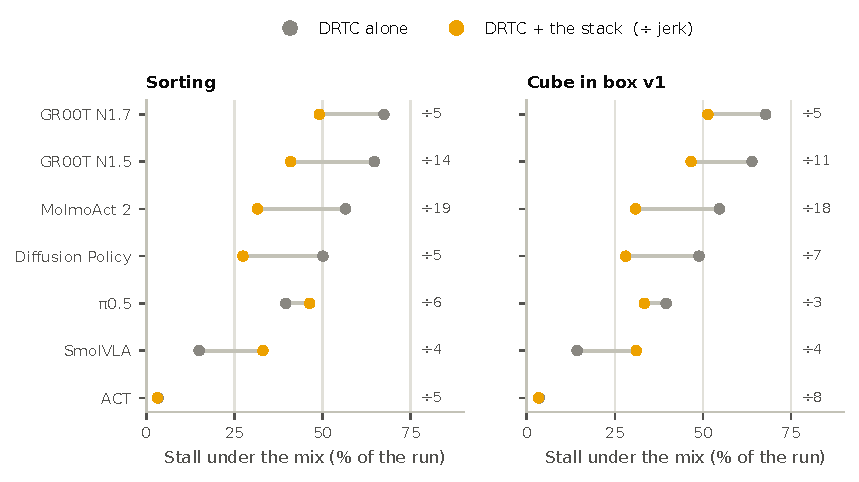
\includegraphics[width=0.84\textwidth]{../report/generated/fig_v2_stack.pdf}
  \caption{Setup v2 E3b: median stall fraction under the fault mix for \drtc{} alone (grey) vs.\ \drtc{} + stack (orange), with jerk reduction factors ($\div$) on the right. The stack cuts stalls on slow policies and reduces jerk 3--20$\times$, while RTC doubles \smolvla{} stalls.}
  \label{fig:v2_stack}
\end{figure*}

\section{Discussion and Limitations}

\subsection{Key Findings}

Our results show that LeRobot~0.7's shipped client fails under faults primarily through its own termination policy rather than policy capability. Raising its limits (patient upstream) prevents aborts, yet still stalls heavily after lost replies because it retries only once on queue depletion. \drtc's advantage over a patient client comes almost entirely from its cooldown re-request, which replaces lost chunks with fresh observations for closed-loop recovery.

Chunk-to-RTT ratio governs smoothing needs more than parameter count: 16-action \groot{} and GR00T~N1.7 stalled for over half of faulted runs without adaptive playback, whereas 100-action ACT stalled 3\% and 50-action \smolvla{} 12--15\%. Moreover, guided RTC trades extra server work for smoother seams; when uncompressed images (2.9~MB, $\approx$260~ms) dominate a 300--450~ms round trip, that added latency costs more stalls than it saves. Finally, fixing bugs on a slow bench link proved critical: three of our four fixes affected cooldown behavior invisible on fast local links, and testing methods individually caught the adverse interaction of soft-stop stale replies.

\subsection{Limitations}

Several honest limitations bound our conclusions:
\begin{itemize}
  \item \textbf{Rising latency regression:} \drtc's cooldown uses recent turnaround history and therefore abandons valid but slower replies under sustained latency rises, stalling more than patient upstream on every policy. A faster-adapting cooldown remains open.
  \item \textbf{Pending robot evaluation (E4):} The first robot run used a fragile shipped baseline (an upper bound on \drtc's benefit) and only two policies on one task; setup~v2 robot trials (E4) and full seven-policy baselines are not yet complete, and $n=10$ trials yield wide Wilson intervals (e.g., \R{main/smolvla/drtc/M1ci} around \R{main/smolvla/drtc/M1}).
  \item \textbf{Bench scope and synthetic faults:} The replay bench measures timing and motion across seven policies and two tasks without task success, and injected faults use shifted synthetic profiles rather than captured WiFi traces.
  \item \textbf{Operational factors:} Operator success judgement was not blinded (mitigated by pre-written rules), shared A100/H200 GPUs introduced contention, and raw image uploads inflated network latency.
\end{itemize}

\section{Conclusion}

We integrated \drtc{} into LeRobot~0.7 with four fixes for slow links and short chunks, built a fault-injection and replay bench covering seven policies and two tasks, and evaluated six smoothing methods under a pre-registered protocol. While \drtc{} restored robot sorting success from 0\% to \R{main/smolvla/drtc/M1}--\R{main/groot/drtc/M1} against the fragile shipped client and cut stalls under packet drops and outages against a patient baseline via cooldown re-requests, it stalled more under rising latency, and guided RTC hurt \smolvla{} on our network-bound link. Future work will complete E4 robot trials, compress camera images, develop an adaptive cooldown for rising latency, extend RTC to relative-action policies, and evaluate an on-robot edge fallback on the Raspberry~Pi~5.

\bibliographystyle{IEEEtran}
\bibliography{../report/references}

\end{document}
